\documentclass{standalone}
\usepackage{tikz,color}
\usetikzlibrary{decorations.pathreplacing}

\begin{document}
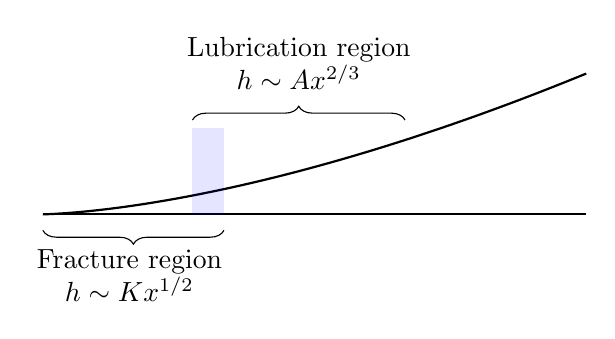
\begin{tikzpicture}

\draw [domain=1:70, samples=50, thick] plot( {0.1*\x}, {0.002*pow(\x,1.6)});

\draw [thick] (0.1,0.003) to (7,0.003);

\path[fill=blue, opacity=0.1] (2,0) rectangle (2.4,1.1);

\draw [ decorate, decoration={brace,mirror,amplitude=5pt}]
(0.1,-0.2) -- ( 2.4, -0.2);
\node at (1.2,-0.6) {Fracture region};
\node at (1.2,-0.95) {$h\sim Kx^{1/2}$};

\draw [ decorate, decoration={brace,amplitude=5pt}]
(2,1.2) -- ( 4.7, 1.2);
\node at (3.35,2.1) {Lubrication region};
\node at (3.35,1.75) {$h\sim Ax^{2/3}$};
\end{tikzpicture}
\end{document}
